%--------------------------------------------------------------------------------------
% Este arquivo contém a sua fundamentação teórica
%--------------------------------------------------------------------------------------
\chapter{Referencial teórico}


\section{Minifoguetes}

Segundo a Brazilian Association of Rocketry (BAR) ou Associação Brasileira de Minifoguetes,  os minifoguetes são definidos como foguetes cujo apogeu seja inferior a $12 \ km$, acima dessa altitude passa a ser considerado um foguete real de grande porte como os foguetes-sonda e os foguetes lançadores. Esses minifoguetes são divididos em duas categorias:


 \begin{itemize}
   \item Foguetemodelo (FM): Que são minifoguetes construídos com motores comerciais inferiores a $160 \ N.s$ de impulso total e que usam materiais não metálicos de densidade baixa como madeira balsa, plásticos, borracha, isopor, fibra de vidro, fibra de carbono etc.  
   
   \item Minifoguete experimental (MFE): minifoguete sem restrições quanto aos materiais empregados e que usa motor-foguete experimental (não comercial). Também é considerado um MFE o minifoguete que usa motor-foguete comercial acima de $160 \ N.s$ de impulso total.

 \end{itemize}




Já o grupo de pessoas que projeta, monta, lança e recupera minifoguetes são divididos em quatro categorias:



 \begin{itemize}
   \item Iniciante:  FM com apogeu inferior a 300 metros.
   
   
   \item Básico: FME com apogeu inferior a 300 metros.
   
   
   \item Intermediário: FM ou FME com apogeu a partir de 300 metros e inferior a 1 km.
   
   
   \item Avançado: FM ou FME com apogeu a partir de 1 km e inferior a 12 km. 
   
 \end{itemize}

 Vale destacar, que o grupo avançado é subdividido de acordo com o máximo apogeu alcançado pelo grupo em $km$, ou seja, $1k$, $2k$, $3k$ etc. O apogeu em $km$ deve ser truncado. Por exemplo, um grupo que tenha conseguido um apogeu de 1700 metros com o seu minifoguete, será denominado grupo de minifoguetes avançado-$1k$ \cite{normas-foguete}.














\newpage
\section{Análise de Sinais e Sistemas}




% ####################################################################################
% ####################################################################################
% ####################################################################################
\subsection{Aliasing}\label{subsec:Aliasing}


O efeito do aliasing é um fenômeno que ocorre quando duas senoides analógicas totalmente diferentes assumem a mesma identidade em tempo discreto,
como é possível ver no exemplo da figura \ref{fig:Aliasing}, que a frequência de $6\ Hz$ está sendo medida como $1\ Hz $ devido a taxa de amostragem  $f_s$ ser apenas $5\ Hz$. Isso normalmente acontece quando a frequência medida se aproxima da frequência de amostragem, causando ambiguidade no processamento digital de sinais  e consequentemente tornando impossível determinar a verdadeira frequência do sinal amostrado \cite{Lathi2018}.


 



\begin{figure}[ht]
    \centering
    \caption{Gráfico efeito aliasing em uma senoide.}
    \begin{center}
        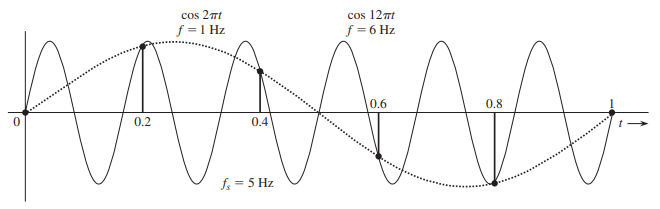
\includegraphics[width=0.9\textwidth]{img/print_aliasing.png}
    \end{center}
    \vspace{-0.5cm}
    \legend{\ABNTEXfontereduzida \textbf{Fonte:} 
    \citeonline[p.~795]{Lathi2018}.}
    

    
    \label{fig:Aliasing}
\end{figure}.

De acordo com o teorema de Nyquist–Shannon onde  $f_s$ é a taxa de amostragem e $f_h$ é a maior frequência a ser processada diz que:


\begin{equation}
    f_s=\frac{1}{T} >2f_h
\end{equation}


Então no exemplo da figura \ref{fig:Aliasing} a taxa de amostragem deveria ser maior do que $12\ Hz$ para que em tempo discreto o sinal de  frequência $6\ Hz$ fosse processada corretamente \cite{Lathi2018}. 






% ####################################################################################
% ####################################################################################
% ####################################################################################
\newpage

\subsection{Conversão analógica-digital}

Um sinal analógico é composto por duas variáveis básicas que são a frequência em Hertz ($Hz$) e a amplitude do sinal em Volts ($v$). Essas duas variáveis podem assumir qualquer valor em uma faixa contínua, ou seja, um sinal analógico pode assumir infinitos valores diferentes de amplitude e de frequência. Já um sinal digital é finito tanto em amplitude e frequência. Se tratando da amplitude, essa pode assumir apenas valores específicos de amplitude chamados de ($L$), que são determinados pela quantidade de bits de resolução ($b$) do conversor A/D \cite{Lathi2018}. 

\begin{equation}\label{eq.conversorAD1}
    2^b = L
\end{equation}

\begin{equation}
    b = \log _{2} L
\end{equation}




Então para converter um sinal analógico em um sinal digital é preciso saber a frequência máxima do sinal a ser medido e utilizar uma taxa de amostragem corretamente como visto na subseção \ref{subsec:Aliasing} e saber a resolução que se deseja ter para a quantização da amplitude do sinal, ou seja, o arredondamento máximo permitido. 





\begin{figure}[ht]
    \centering
    \caption{Onda senoidal quantizada em 4 bits.}
    \begin{center}
        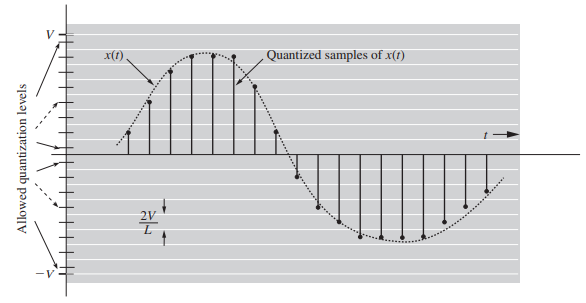
\includegraphics[width=0.9\textwidth]{img/print_Conversao_AD1.png}
    \end{center}
    \vspace{-0.5cm}
    \legend{\ABNTEXfontereduzida \textbf{Fonte:} 
    \citeonline[p.~800]{Lathi2018}.}
    

    
    \label{fig:AD1}
\end{figure}








.

Tendo como exemplo um conversor A/D de $4$ bits, esse possuí $L =2^4= 16$ estados de amplitude diferente. Como mostra o gráfico da figura \ref{fig:AD1}, o sinal analógico foi repartido em 16 níveis de amplitude diferentes e cada nível foi convertido em um código binário como mostra a tabela da figura \ref{fig:AD2}.
 




\begin{figure}[ht]
    \centering
    \caption{Tabela conversão Analógico Digital 4 bits.}
    \begin{center}
        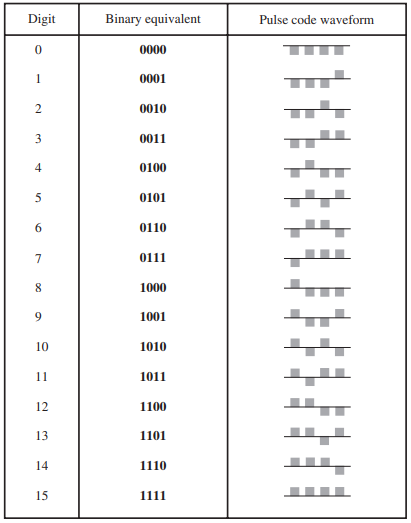
\includegraphics[width=0.5\textwidth]{img/print_Conversao_AD2.png}
    \end{center}
    \vspace{-0.5cm}
    \legend{\ABNTEXfontereduzida \textbf{Fonte:} 
    \citeonline[p.~800*]{Lathi2018}.}
    

    
    \label{fig:AD2}
\end{figure}.


Supondo que a tensão de pico a pico ($VPP$) do sinal fosse de $4 \ v$, então a tensão de entrada do conversor teria de ser no mínimo igual ou maior que $4 \ v$, mas vamos assumir por padrão 5 volts. Utilizando a equação \ref{eq.conversorAD1} se conclui que o conversor apresenta $L=16$ estados de quantização. Então para saber a resolução basta  dividir a tensão máxima por L.

\begin{equation}
    \frac{5 \ v}{2^4}=0,3125 \ v
\end{equation}

Com isso podemos observar que um conversor de 4 bits tem como escala $0,312 \ v$. Caso a aplicação necessitasse medir $0,1 \ v$ esse conversor de 4 bits iria ler como $0 \ v$, substituindo o conversor de 4 bits por um de 8 bits, por exemplo, esse teria uma escala de $0,0195 \ v$ e para medir $0,1V$ iria apresentar um erro de $0,00234 \ v$. Caso esse erro não fosse permitido precisaríamos de um conversor A/D com uma resolução ainda maior \cite{Lathi2018}. 








% ####################################################################################
% ####################################################################################
% ####################################################################################

\newpage

\subsection{Razão sinal-ruído}

Todas as medidas analíticas possuem dois componentes. Um sinal que carrega a informação útil e o outro componente que é formado por informações indesejadas que é chamado de Ruído. A razão sinal ruído, do inglês Signal to Noise Ratio (SNR), é mais usada do que o valor apenas do ruído. Isso porque, o valor SNR indica o quanto de impureza o sinal desejado possuí, como é mostrado no exemplo da figura \ref{fig:RelacaoSinalRuido}a em comparação ao sinal teórico mostrado na figura \ref{fig:RelacaoSinalRuido}b \cite[p.~98]{principioAnaliseInstrumental}.






 




\begin{figure}[ht]
    \centering
    \caption{(a) Efeito do ruído sobre uma medida de corrente contínua de $ 0,9*10^{-15}A$. (b) Média das flutuações.}
    \begin{center}
        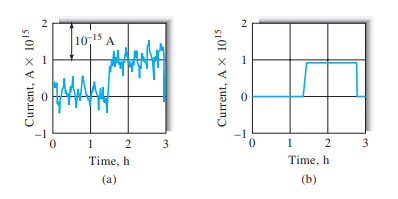
\includegraphics[width=0.7\textwidth]{img/print_relacao_Sinal-Ruido.png}
    \end{center}
    \vspace{-0.5cm}
    \legend{\ABNTEXfontereduzida \textbf{Fonte:} 
    \citeonline[p.~99]{principioAnaliseInstrumental}.}
    

    
    \label{fig:RelacaoSinalRuido}
\end{figure}.
 
 

 
 



A relação sinal ruído é expressa em decibéis. Como se trata de uma escala logarítmica, o SNR é obtido através da seguinte forma: 


\begin{equation}
    P_{sinal,dB}=10 \log(P_{sinal})
\end{equation}



\begin{equation}
    P_{ruído,dB}=10 \log(P_{ruído})
\end{equation}



\begin{equation}
   SNR_{dB} = 10 \log(\frac{P_{sinal}}{P_{ruído}} )
\end{equation}


% ####################################################################################
% ####################################################################################
% ####################################################################################














\newpage



\section {Sensores Inerciais}


 De acordo com a segunda lei de Newton conhecida como princípio fundamental da dinâmica, afirma que a força resultante ($ F $) que atua sobre um corpo é igual ao produto de sua massa ($m$) pela aceleração ($a$). Se rearranjarmos a equação temos:
 
 \begin{equation}
    a = \frac{F}{m}
\end{equation}
 
 Existindo uma relação entre a aceleração, a velocidade ($v$) e a posição ($x$) do objeto por meio de suas derivadas:
  \begin{equation}
    v = f'(x) = \frac{dx}{dt}
\end{equation} 

  \begin{equation}
    a = v'(x) = \frac{d^2x}{dt^2}
\end{equation} 
 
 Apesar de existir essa relação entre as grandezas, a utilização de derivadas em ambientes que contem ruído para se obter a velocidade e a aceleração a partir da derivada da posição terá como resultado erros elevados. Por causa disso, a velocidade e aceleração não são derivadas de sensores de posição, mas sim por sensores inerciais \cite[380]{ModernSensors}.


Os sensores inerciais têm como finalidade a obtenção completa do movimento de um objeto sólido por meio de duas grandezas físicas vetoriais acessíveis que são a aceleração e a velocidade ao redor dos três eixos ortogonais X, Y e Z. Os principais sensores inerciais existentes são os acelerômetros utilizados para se obter a aceleração em $a  = m/s^2$ e os giroscópios utilizados para obtenção das velocidades angulares em $\omega= rad/s $ \cite[p.~527]{Korvink2006}.




% ####################################################################################
% ####################################################################################
% ####################################################################################


%#############################################
%  Esta Pronto     v
%#############################################



\newpage
\subsection{Acelerômetro}


Os acelerômetros lineares pertencem à classe dos sensores inerciais que não requerem
referência a um sistema de coordenadas estacionário. Normalmente se utiliza três acelerômetros ortogonais com o intuito de medir a aceleração linear em cada eixo do espaço incluindo a gravidade. Assim, um acelerômetro típico deve responder a várias formas de acelerações desde movimento lentos, fortes a impactos e vibrações. Um fato interessante é que ao processar os sinais desses dispositivos é possível rastrear a posição e orientação de um objeto em movimento \cite{ModernSensors}.

 Os acelerômetros mecânicos consistem em um sistema massa-mola com um sensor de deslocamento interno como mostra a figura \ref{fig:ModernSensors}a. Como a massa de prova ($m$), a constante elástica da mola ($k$), e o valor do deslocamento ($\Delta x$)  provocado pela aceleração são conhecidos, a obtenção do valor da aceleração se torna possível utilizando as equações de Hooke e a segunda lei de Newton.


\begin{equation}
    F = -k\cdot\Delta x
\end{equation}


\begin{equation}
    a =\frac{-k\cdot\Delta x}{m}
\end{equation}


 

\begin{figure}[ht]
    \centering
    \caption{(a) Conceito de acelerômetro mecânico linear. (b) Diagramas de tempo.}
    \begin{center}
        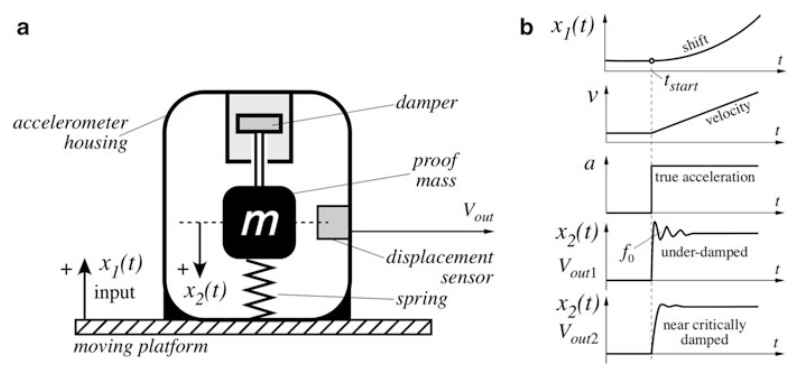
\includegraphics[width=1\textwidth]{img/print_acelerometro_conceito.png}
    \end{center}
    \vspace{-0.5cm}
    \legend{\ABNTEXfontereduzida \textbf{Fonte:} 
    \citeonline[p.~393]{ModernSensors}.}
    

    
    \label{fig:ModernSensors}
\end{figure}.
\newpage



 Um bom acelerômetro deve ter dois parâmetros bem identificados que são a frequência ressonante ou frequência natural e uma faixa de resposta de frequência plana onde a medição da aceleração se torna mais precisa sem distorções provocadas pelas características de frequência do
acelerômetro como é mostrado na figura \ref{fig:grafico_acelerometro}. No entanto, quando a frequência medida é muito maior do que o limite de largura de banda de operação do acelerômetro, um filtro passa-baixa é necessário para filtrar o sinal \cite{ModernSensors}.
 
 
 



\begin{figure}[ht]
    \centering
    \caption{Uma frequência-resposta de um acelerômetro onde f\textsubscript{0} é a frequência natural e f\textsubscript{ref} é a frequência de referência.}
    \begin{center}
        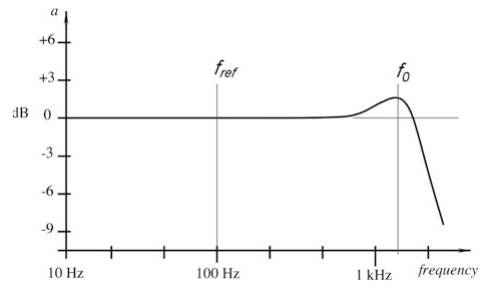
\includegraphics[width=0.7\textwidth]{img/print_grafico_resposta_do_acelerometro.png}
    \end{center}
    \vspace{-0.5cm}
    \legend{\ABNTEXfontereduzida \textbf{Fonte:} 
    \citeonline[p.~396]{ModernSensors}.}
    

    
    \label{fig:grafico_acelerometro}
\end{figure}.

%#############################################
%  Esta Pronto     ^
%#############################################










Como o sistema apresenta uma massa, uma  mola e um amortecedor interno, com a finalidade de consumir a energia fornecida a mola pela aceleração, fazendo com que a massa volte a sua posição inicial (sem aceleração). O sistema irá se comportar como um oscilador, tendo características estáticas e dinâmicas. Uma das características estáticas mais importantes é a sensibilidade estática (S) dada por:


\begin{equation}
    S=\frac{m}{k} = \frac{1}{\omega_0^2} = \frac{1}{(2 \pi f_0)^2}
    \label{9.19_equacao_sensibilidade_estatica}
\end{equation} 

Onde o S é inversamente proporcional ao quadrado da frequência natural ($f_0$) em Hz. Outra característica estática é o coeficiente de amortecimento b que é definido através do parâmetro $\zeta$ chamado de razão de amortecimento

\begin{equation}
    b = 2 \zeta\sqrt{km}   
    \label{9.21_equacao_coeficiente_amortecimento}
\end{equation} 




Levando em conta todas as forças que atuam na massa de prova (força de inércia, força da mola, e amortecimento) a equação diferencial linear de segunda ordem que descreve esse sistema é:


\begin{equation}
    m\frac{d^2x_2}{dt^2}+b(\frac{dx_2}{dt}-\frac{dx_1}{dt})+k(x_2-x_1)=0
    \label{9.22_equacao_diferencial}
\end{equation} 


Chamando $ x_2 - x_1 = \Delta x $ que é o deslocamento relativo da massa de prova sendo traduzida pelo sensor de deslocamento como uma tensão de saída V\textsubscript{out}. Então, a equação \ref{9.22_equacao_diferencial} pode ser reescrito como

  \begin{equation}
    m\frac{d^2\Delta x}{dt^2}+b\frac{d\Delta x}{dt}+k\Delta x=-ma=-F
    \label{9.23_equacao_diferencial}
\end{equation} 


Tendo como solução da equação \ref{9.23_equacao_diferencial} para um deslocamento relativo $\Delta x(t)$ :


\begin{equation}
    \Delta x(t) = Be^{-\zeta\sqrt{t\frac{k}{m}}}\sin{(2\pi f_dt+\varphi )}  - Sa 
    \label{9.24_equacao}
\end{equation} 





Onde o fator B e o deslocamento de fase $\varphi$, dependem da posição da massa de prova no
momento do início da aceleração.
A frequência amortecida $f_d$ é diferente da frequência natural $f0$ e só é valida para $\zeta<1$ definida como:


\begin{equation}
    f_d = f0\sqrt{1-\zeta^2} 
    \label{9.25_equacao}
\end{equation} 


Várias conclusões podem ser tiradas da solução \ref{9.24_equacao}, como a saída ter uma
natureza oscilatória decadente caracterizada pela primeira soma, sendo que a taxa de decaimento é exponencial com uma constante de tempo:


\begin{equation}
    \tau = \frac{1}{\zeta}\sqrt{\frac{m}{k}}
    \label{9.26_equacao_Constante_tempo}
\end{equation} 


É observável que pela equação \ref{9.26_equacao_Constante_tempo}, quanto maior a razão de amortecimento $\zeta$, mais rápido as oscilações indesejadas desaparecem. Porém, a medida que $\zeta$  fica maior que 1, o acelerômetro fica menos sensível e consequentemente mais lento. A melhor condição é quando ($\zeta \approx 1$), apresentando uma resposta crítica ou quase criticamente amortecida se comportando da forma mais aproximada da verdadeira aceleração como é mostrado no gráfico de $V_{out2}$ da figura \ref{fig:ModernSensors}b \cite{ModernSensors}. 


Vale ressaltar que a sensibilidade de um acelerômetro é a razão de uma saída elétrica para a entrada mecânica, expresso em volts por unidade de aceleração. Por exemplo, a sensibilidade pode ser especificada como $1 V/g$ (unidade de aceleração: $ g = 9,806 \ m/s^2$ ao nível do mar. Ela é tipicamente medida em uma única frequência de referência na forma de onda senoidal \cite{Korvink2006}.


\newpage











% ####################################################################################
% ####################################################################################
% ####################################################################################


\subsection{Giroscópio}


 

Os giroscópios pertencem à classe dos sensores rotativos inerciais. Este sensor é um dispositivo responsável por "guardar a direção", isso significa que ele produz um sinal na saída sempre que a velocidade angular se desvia de zero, o que acontece quando a plataforma começa a girar. O funcionamento do giroscópio tem como base o princípio fundamental da conservação do momento angular, que diz que em qualquer sistema de partículas, o momento angular total do sistema em relação a qualquer ponto fixo no espaço permanece constante, desde que nenhuma força externa aja sobre o sistema. Um sensor inercial rotativo completo normalmente contém três giroscópios de taxa ortogonal, medindo as velocidades angulares em cada eixo. \cite{ModernSensors}. 

Um giroscópio mecânico é composto por um disco maciço livre para girar em torno de um eixo de rotação, que está confinado dentro de uma estrutura que é livre para girar em torno de um ou dois eixos como mostra a figura \ref{fig:Giroscopio_Conceitual}. Assim, dependendo do número de eixos rotativos, um giroscópio pode ser de um ou dois graus de liberdade. 


 


\begin{figure}[ht]
    \centering
    \caption{Giroscópio mecânico conceitual.}
    \begin{center}
        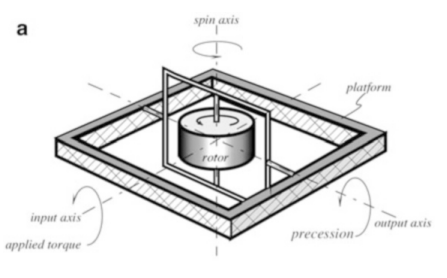
\includegraphics[width=0.8\textwidth]{img/print_giroscopio_mecanico_conceitual.png}
    \end{center}
    \vspace{-0.5cm}
    \legend{\ABNTEXfontereduzida \textbf{Fonte:} 
    \citeonline[p.~386]{ModernSensors}.}
    

    
    \label{fig:Giroscopio_Conceitual}
\end{figure}.



Esse dispositivo inercial rotativo, pode ser feito para fornecer um torque (ou sinal de saída) que é proporcional a velocidade angular em torno de um eixo perpendicular ao eixo de rotação.
Quando o rotor gira livremente, ele tende a preservar sua posição axial. Se a plataforma do giroscópio gira em torno do eixo de entrada, o giroscópio desenvolverá um torque em torno de um eixo perpendicular (saída), girando assim, seu eixo de rotação em torno do eixo de saída. Esse fenômeno é chamado de precessão de um giroscópio, e isso pode ser explicado pela lei de Newton do movimento para rotação, onde a taxa de tempo de mudança do momento angular sobre qualquer eixo é igual ao torque aplicado em torno do eixo dado. Ou seja, quando um torque T é aplicado em torno do eixo de entrada, e a velocidade $\omega$ do rotor é mantida constante, o momento angular do rotor pode ser alterado apenas girando a projeção do eixo de rotação em relação ao eixo de entrada. 


\begin{equation}
    T = I\omega \Omega
    \label{equação_9.10}
\end{equation}


Como mostra a equação \ref{equação_9.10}, a taxa de rotação do eixo de rotação em torno do eixo de saída é proporcional ao torque aplicado, onde $\Omega$ é a velocidade angular sobre o eixo de saída e I é a inércia de um giroscópio em torno do eixo de rotação. Se tratando da precisão de um giroscópio mecânico, esta depende muito dos efeitos que podem causar torques adicionais indesejados que pode causar desvios. As fontes destes problemas são o atrito, rotor desbalanceado, efeitos magnéticos, etc \cite{ModernSensors}.

Outros métodos para detectar uma direção e velocidade angular foram desenvolvidos, por exemplo, o Sistema de Posicionamento Global (GPS), mas, ele simplesmente não pode ser empregado no espaço, debaixo d'água, em túneis, dentro de prédios, ou sempre que o tamanho e custo forem de uma importância primordial. Além disso, a resolução espacial do GPS quase não é suficiente para muitos dispositivos  e isso torna o uso de um giroscópio bastante relevante principalmente em mísseis e foguetes \cite{Korvink2006}. 














% ####################################################################################
% ####################################################################################
% ####################################################################################


\section{Magnetômetro}


O sensor magnetômetro atua como uma bússola digital sendo utilizado para aferir a intensidade, direção e sentido de campos magnéticos em sua proximidade. Na ausência de campos eletromagnéticos locais fortes, essas medições serão do ambiente, no caso, detectando o campo magnético da Terra e permitindo assim que o sensor determine a sua direção em relação ao Polo Norte geomagnético. Vale lembrar que a  direção geomagnética e a verdadeira direção em relação ao Polo Norte geográfico pode variar por várias dezenas de graus, dependendo da localização no planeta. Normalmente esse tipo de sensor retorna a intensidade do campo eletromagnético em Microtesla ($\micro T$), nas três coordenadas X,Y e Z \cite{Jepson2011}.

\newpage







% ####################################################################################
% ####################################################################################
% ####################################################################################







% ####################################################################################
% ####################################################################################
% ####################################################################################









% ####################################################################################
% ####################################################################################
% ####################################################################################
\newpage
\section {INSTRUMENTAÇÃO ELETRÔNICA}



\subsection{Sensor BNO055}\label{subsec:BNO055}



O BNO055 é um System in Package (SiP), desenvolvido pela empresa BOSCH. Esse circuito integrado contém um acelerômetro triaxial de 14 bits de resolução, um Giroscópio de 16 bits de resolução com alcance de ±2000 graus por segundo, um sensor geomagnético triaxial e um microcontrolador córtex M0+ de 32 bits executando o software de fusão de sensores Bosch Sensortec, que é responsável por corrigir e integrar as informações dos 3 sensores em um único encapsulamento \cite{BOSCH2021}.  


 

\begin{figure}[ht]
    \centering
    \caption{Sensor BNO055 com os circuitos adicionais.}
    \begin{center}
        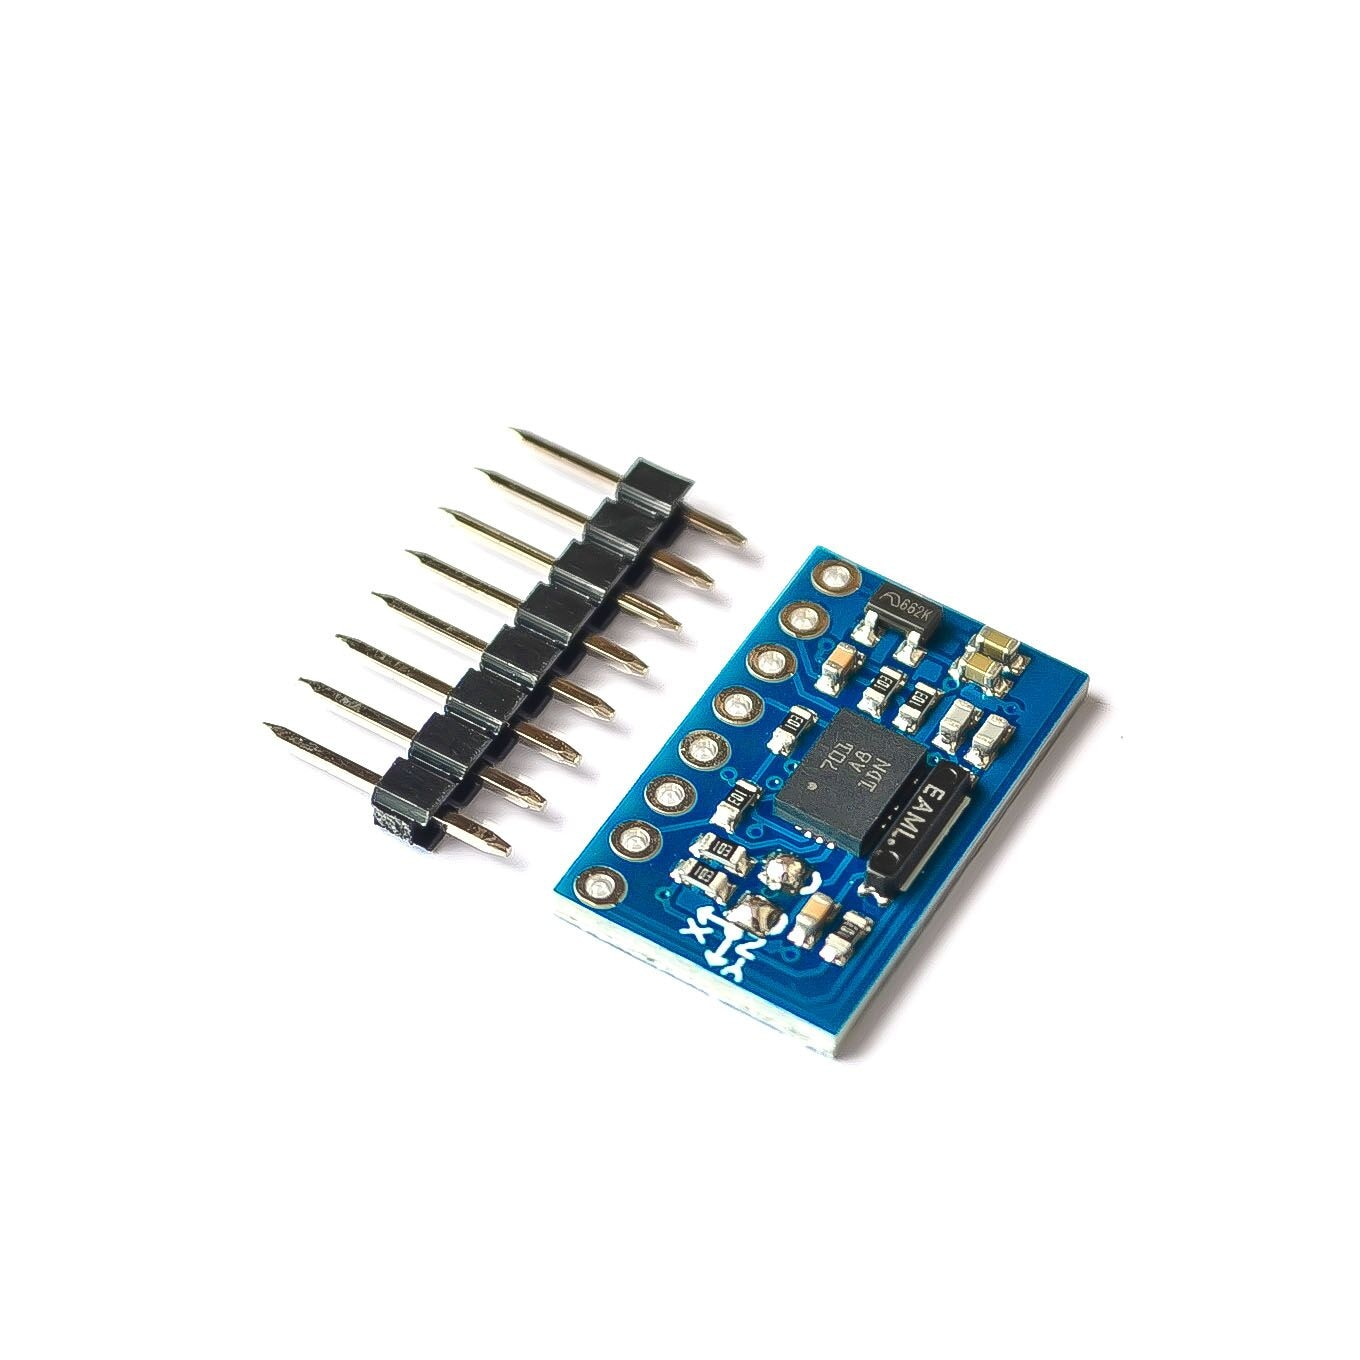
\includegraphics[width=0.50\textwidth]{img/Sensor BNO055.jpg}
    \end{center}
    \vspace{-0.5cm}
    \legend{\ABNTEXfontereduzida \textbf{Fonte: Site Aliexpress}}
    \label{fig:BNO055}
\end{figure}.




O  Circuito Integrado CI montado no modulo da figura \ref{fig:BNO055} possui quatro vantagens em relação a utilização de três sensores separados:


 \begin{enumerate}
   \item Redução de espaço e peso adicionado ao foguete;
   \item Redução de processamento do microcontrolador principal;
   \item Redução de falhas de comunicação devido a redução de componentes eletrônicos na placa de circuito impresso PCB;
   \item Redução da complexidade de desenvolvimento de software e hardware.
 \end{enumerate}


















% ####################################################################################
% ####################################################################################
\newpage
\subsection{Sensor BME280}


O BME280 é um sensor três em um desenvolvido pela empresa BOSCH. Esse dispositivo apresenta um sensor de pressão atmosférico com range de $300$ à $1100 \ hPa$, um sensor de umidade com range de $0$ à $100\% $ umidade relativa e um sensor de temperatura com range de $-40$ à $+85 \ \celsius$ \cite{BMP280}.

\begin{equation}
    P = \rho gh
     \label{equação_10}
\end{equation}


De acordo com a equação \ref{equação_10}, onde $P = pressão$, $\rho =  densidade \ do \ ar$ e $h = altura $. É observável que a densidade do ar interfere na pressão medida, de acordo com a lei dos gases, a temperatura e umidade interferem na densidade do gases, logo o sensor BME280 visto na figura \ref{fig:BMP280} se torna um altímetro mais preciso do que o BMP280  que só conta com o sensor de pressão atmosférica e consequentemente não pode corrigir os efeitos causados na pressão pela temperatura e umidade do ar  \cite[p.~465]{Halliday2010}.




 



\begin{figure}[ht]
    \centering
    \caption{Sensor BME280 com os circuitos adicionais.}
    \begin{center}
        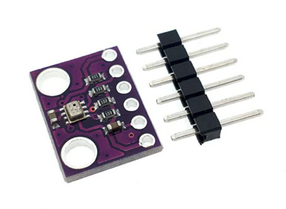
\includegraphics[width=0.50\textwidth]{img/BMP280.png}
    \end{center}
    \vspace{-0.5cm}
    \legend{\ABNTEXfontereduzida \textbf{Fonte: Site Aliexpress}}
    %\citeonline{BNO055}.}
    \label{fig:BMP280}
\end{figure}.

Assim como o sensor BNO055 apresentado na subseção \ref{subsec:BNO055},  o  Circuito Integrado CI montado no modulo da figura \ref{fig:BMP280} possui vantagens em relação a utilização de três sensores separados:


 \begin{enumerate}
   \item Redução de espaço e peso adicionado ao foguete;
   \item Redução de falhas de comunicação devido a redução de componentes eletrônicos na placa de circuito impresso PCB;
   \item Redução da complexidade de desenvolvimento de hardware.
 \end{enumerate}






% ####################################################################################
% ####################################################################################
\newpage
\subsection{GPS NEO-6M}

O modulo NEO-6M é um sistema de posicionamento Global (GPS) que tem suporte até 50 canais de satélites geoestacionários, taxa de navegação máxima até $5 \ Hz$, precisão horizontal de $2,5 \ m$ e podendo operar em uma faixa de $-40$ à $+80 \ \celsius$  \cite{NEO-6M}. Esse modulo por padrão retorna o seguinte protocolo NMEA de mensagens:
 \begin{enumerate}
    \item GSV = O número de satélites disponíveis, o número de identificação por satélite, elevação, azimute e valores SNR.
    \item RMC = Dados de hora, data, posição, curso e velocidade. 
    \item GSA = Modo de operação do receptor GPS, satélites usados na solução de posição,"' e valores DOP.
    \item GGA = Dados de tempo, posição e correção dos dados.
    \item GLL = Latitude, longitude, tempo UTC de correção de posição e status 
    \item VTG = Informações de curso e velocidade relativas ao solo.
 \end{enumerate}



Como mostra a figura \ref{fig:GPSNEO6M}, este modulo por ser pequeno e leve tem a vantagem de não impactar demasiadamente no desempenho do foguete. Vale destacar que apesar deste modulo apresentar uma taxa de atualização baixa na ordem de $5 \ Hz$, não é tão relevante para o projeto adicionar um GPS com uma taxa de atualização mais alta como é o caso do NEO-7M com taxa de $10 \ Hz$ ou NEO-8M com taxa de $15 \ Hz$ e consequentemente aumentar o custo do projeto, já que sua função principal é ajudar na localização do foguete. 


 



\begin{figure}[ht]
    \centering
    \caption{GPS NEO-6M com os circuitos adicionais e antena.}
    \begin{center}
        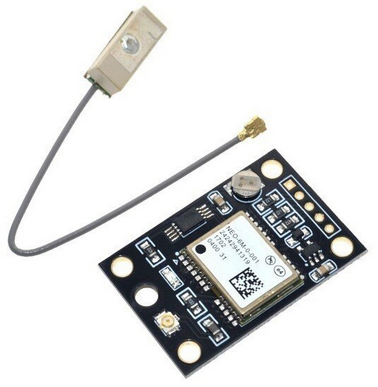
\includegraphics[width=0.40\textwidth]{img/NEO-6M GPS.png}
    \end{center}
    \vspace{-0.5cm}
    \legend{\ABNTEXfontereduzida \textbf{Fonte: Site Aliexpress}}
    %\citeonline{BNO055}.}
    \label{fig:GPSNEO6M}
\end{figure}.















\begin{comment}
Este é um comentário de múltiplas linhas.
Com certeza útil para esconder partes grandes de texto ainda não revisadas.
Ou para encontrar um problema do seu código LaTeX que não compila.






\alpha α
\beta β
\gamma e \Gamma γ e Γ
\delta e \Delta δ e ∆
\epsilon e \varepsilon ǫ e ε
\zeta ζ
\eta η
\vartheta, \theta e \Theta θ, θ e Θ
\iota ι
\kappa κ
\lambda e \Lambda λ e Λ
\mu μ
\nu ν
\xi e \Xi ξ e Ξ
\pi e \Pi π e Π
\rho e \varrho ρ e ̺
\sigma, \varsigma e \Sigma σ, ς e Σ
\tau τ
\upsilon e \Upsilon υ e Υ
\phi, \varphi e \Phi φ, φ e Φ
\chi χ
\psi e \Psi ψ e Ψ
\omega e \Omega ω e Ω




\end{comment}









% ####################################################################################
% ####################################################################################
% ####################################################################################
\newpage
\subsection{Radio Lora^{TM}}




% ###############################################

O modulo de rádio frequência RF lora é uma boa escolha devido as suas características benéficas como uma taxa de transferência variável o que possibilita a troca de largura de banda por alcance e também pelo seu custo benefício. Por padrão ele apresenta uma taxa de transferência de dados de $2,4 \ kbps$ o que é mais do que suficiente para transmitir os dados dos sensores do foguete para o solo \cite{EBYTE2019}. 

Como mostra a figura \ref{fig:RadioLora} esse modulo é relativamente pequeno e leve, se tornando uma escolha ideal por não interferir no desempenho do foguete. Além disso, segundo o datasheet o modulo pode atingir um alcance de até $8 \ km$ o que significa que poderá suprir as necessidades tanto de foguetemodelos de porte iniciante e intermediário.






\begin{figure}[ht]
    \centering
    \caption{Radio Lora E32-433T30D.}
    \begin{center}
        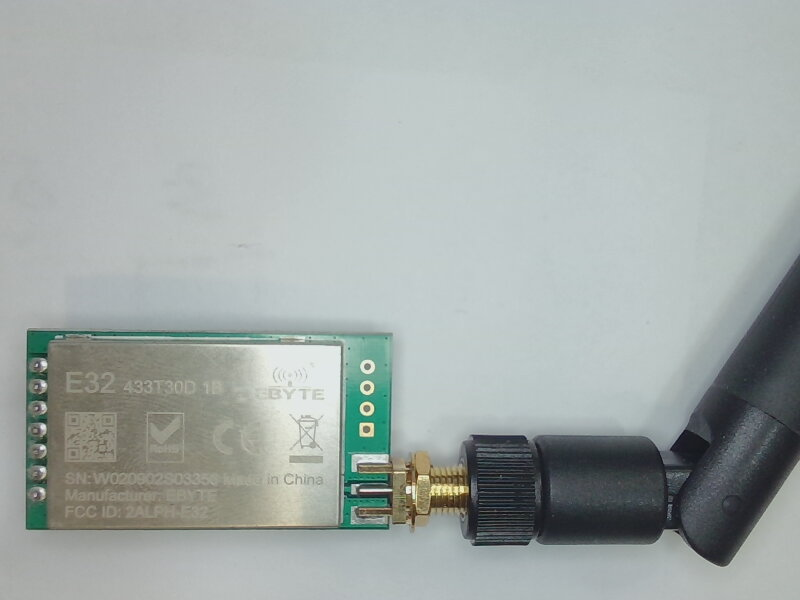
\includegraphics[width=0.6\textwidth]{img/Modulo RF Lora.jpg}
    \end{center}
    \vspace{-0.5cm}
    \legend{\ABNTEXfontereduzida \textbf{Fonte: O autor.} 
    }
   \label{fig:RadioLora}
\end{figure}

% ###############################################
Como mostra a tabela \ref{tab:radioLora} retirado do datasheet é possível ver as principais características do modulo entre elas a frequência de transmissão trabalhando dentro de $410 \ MHz$ até $441 \ MHz$, por padrão $433 \ MHz$, que é uma frequência de grande interesse já que ela não sofre tamanha interferência causada por inúmeros outros dispositivos operando na mesma faixa de frequência como é o caso de aparelhos em $2,4 GHz$.



\begin{table}[!htb]
	\centering
	\caption{\label{tab:radioLora} Especificações do Modulo E32- 433T30D.}
	\begin{adjustbox}{max width=\textwidth}
%		\begin{tabular}{@{} p{5cm} |c|c|c|c|@{}}
        \begin{tabular}{@{} p{2cm} |c|c|c|c|c|c}
		\toprule
		\textbf{Model} & \textbf{Core IC} & \textbf{Frequency Hz} & \textbf{Tx Power dBm} & \textbf{Distance km} & \textbf{Date Rate} & \textbf{Interfece}\\ \hline

		\textbf{E32- 433T30D} &
			SX1278 & 433M & 30 & 8 & 0.3k~19.2k & SMA-K
%		\\ \hline

		\\ \bottomrule
	\end{tabular}
	\end{adjustbox}
	\legend{\textbf{Fonte:} \citeonline[p.~17]{EBYTE2019}}
\end{table}









% ####################################################################################
% ####################################################################################
% ####################################################################################

\newpage
%\section{Seção de exemplo 1 - Como fazer citações}
\begin{comment}
Existem vários tipos de citações...
















%\imagem{0.15}{missil_balistico_V2}{Missil balistico V2 sendo preparado para lançamento em %Cuxhaven, na Alemanha, 15 de  outubro de 1945.}{AP IMAGES, 2022}

%A figura \ref{img:missil_balistico_V2} é um exemplo do outro tipo de figura abordada aqui, chamada %de figura composta. Esta figura é composta de outras subfiguras.



%\begin{figure}[!htb]
%\centering
 %   \caption{\label{img:missil_balistico_V2} Missil balistico V2 sendo preparado para lançamento em Cuxhaven, na Alemanha, 15 de  outubro de 1945.}

  %  \legend{\textbf{Fonte:AP IMAGES, 2022}\citeonline{ACESSADO EM: https://www.apimages.com/metadata/Index/Watchf-AP-I-DEU-APHSL37937-Post-WWII-germany-V2-/e918f669900d409caba6ccabee822d81/100/0}}
%\label{fig:dag}
%\end{figure}





%\begin{figure}[!htb]
%\centering
 %   \caption{\label{img:figura1} Exemplo de figura composta}
  %  \subcaptionbox{\label{img:subfigura1} Subfigura 1}{
\includegraphics[scale=.1]{img/placeholder}}\qquad
   % \subcaptionbox{\label{img:subfigura2} Subfigura 2}{
\includegraphics[scale=.1]{img/placeholder}}
%    \vspace{1.5em}
%    \legend{\textbf{Fonte:} \citeonline{SUA-REFERENCIA}}
%\label{fig:dag}
%\end{figure}




Para referenciar uma figura deve ser usada comando \textbackslash ref\{img:<label ou nome do arquivo>\}, como exemplo, estamos referenciando a figura \ref{img:placeholder}. Isso vale tanto para figuras simples quanto para as compostas, como por exemplo as figuras \ref{img:subfigura1} e \ref{img:subfigura2}. Ao inserir uma figura, ela é automaticamente identificada e incluída no elemento pré-textual da lista de figuras.





%\lipsum[5-10]

Colocar citações longas entre \textbackslash begin\{citacao\} e \textbackslash end\{citacao\}, exemplo: 

\begin{citacao}
``\lipsum[1]''

\cite{REFERENCIA}
\end{citacao}





\section{Seção de exemplo 2 - Como inserir figuras}

Neste trabalho iremos exemplificar duas formas de se inserir figuras no Latex. O primeiro método insere, no documento, uma figura simples por meio do comando:

\textbackslash imagem\{ Escala \}\{ Arquivo sem extensão \}\{ Descrição \}\{ Fonte \}

\textbf{Obs.:} A fonte pode ser uma citação do tipo  \textbackslash citeonline\{\}.

A figura \ref{img:placeholder} é um exemplo deste método.

%--------------------------------------------------------------------------------------
% Esse é um exemplo de figura simples
%--------------------------------------------------------------------------------------
\imagem{0.15}{placeholder}{Uma figura simples}{O autor}

A figura \ref{img:figura1} é um exemplo do outro tipo de figura abordada aqui, chamada de figura composta. Esta figura é composta de outras subfiguras.
%--------------------------------------------------------------------------------------
% Esse é um exemplo de figura composta de outras subfiguras
%--------------------------------------------------------------------------------------
\begin{figure}[!htb]
\centering
    \caption{\label{img:figura1} Exemplo de figura composta}
    \subcaptionbox{\label{img:subfigura1} Subfigura 1}{
\includegraphics[scale=.1]{img/placeholder}}\qquad
    \subcaptionbox{\label{img:subfigura2} Subfigura 2}{
\includegraphics[scale=.1]{img/placeholder}}
    \vspace{1.5em}
    \legend{\textbf{Fonte:} \citeonline{SUA-REFERENCIA}}
\label{fig:dag}
\end{figure}

%\begin{figure}[!htb]
%\centering
%    \caption{\label{img:telas} Telas da aplicação cliente}
%    \subcaptionbox{\label{img:inicial} Abertura}{\includegraphics[scale=.12]{img/APP/inicial}}\qquad
%    \subcaptionbox{\label{img:login} \textit{Login}}{\includegraphics[scale=.12]{img/APP/login}}\qquad
%    \subcaptionbox{\label{img:cadastro} Cadastro}{\includegraphics[scale=.12]{img/APP/cadastro}}\qquad
%    \subcaptionbox{\label{img:hist-rel}Sobre}{\includegraphics[scale=.12]{img/APP/sobre}}\\
%    \vspace{1.5em}
%    \subcaptionbox{\label{img:dados_atuais}Dados atuais}{\includegraphics[scale=.15]{img/APP/atual}}\qquad
%    \subcaptionbox{\label{img:hist-time}Seleção de período}{\includegraphics[scale=.15]{img/APP/periodo}}\qquad
%    \subcaptionbox{\label{img:hist-rel}Exibir histórico}{\includegraphics[scale=.15]{img/APP/historico}}\\
%    \vspace{2.5em}
%    \legend{\textbf{Fonte:} O Autor}
%\label{fig:dag}
%\end{figure}

Para referenciar uma figura deve ser usada comando \textbackslash ref\{img:<label ou nome do arquivo>\}, como exemplo, estamos referenciando a figura \ref{img:placeholder}. Isso vale tanto para figuras simples quanto para as compostas, como por exemplo as figuras \ref{img:subfigura1} e \ref{img:subfigura2}. Ao inserir uma figura, ela é automaticamente identificada e incluída no elemento pré-textual da lista de figuras.




\section{Seção de exemplo 3 - Sobre tabelas}

As tabelas em Latex são deveras capciosas, por isso não serão abordadas em sua completude neste documento.

Há um site que possui uma ferramenta interessante para ser utilizada na construção tabelas em Latex.

\centerline{\href{https://www.tablesgenerator.com/}{ O Tables Generator } <-- Isto é um \textit{link} :D}

Contudo, busquem entendimento sobre o assunto, pois tabelas são elementos textuais importantes e enriquecem muito o texto, quando bem construídas.

A tabela \ref{tab:crossplatform} é um exemplo de como uma tabela pode ser construída, assim como a tabela do anexo \ref{anex:anexo1}.

\begin{table}[!htb]
	\centering
	\caption{\label{tab:crossplatform} Tipos de aplicações e abordagens preferenciais.}
	\begin{adjustbox}{max width=\textwidth}
		\begin{tabular}{@{} p{5cm} |c|c|c| @{}}
		\toprule
		\textbf{Código da Aplicação} & \textbf{Web} & \textbf{Híbrida} & \textbf{Interpretada / Compilação Cruzada} \\ \hline

		\textbf{Aplicações baseadas em dados providos por um servidor} &
			3 & 2 & 1
		\\ \hline

		\textbf{Aplicações independentes} & 1 & 2 & 3\\ \hline

		\textbf{Aplicações baseadas em sensores e processamento de dados no dispositivo} & 1 & 2 & 3\\ \hline

		\textbf{Aplicações baseadas em sensores e processamento de dados no servidor} & 1 & 3 & 2\\ \hline

		\textbf{Aplicações Cliente-Servidor} & 1 & 3 & 2 \\ \bottomrule
	\end{tabular}
	\end{adjustbox}
	\legend{\textbf{Fonte:} \citeonline{raj2012study} (Traduzido)}
\end{table}

Também é possível criar quadros, que são ligeiramente diferente de tabelas. Acompanhe o exemplo no Quadro \ref{qua:confusionmatrix}

\begin{quadro}
	\centering
	\caption{\label{qua:confusionmatrix}Exemplo de matriz de confusão}
	\begin{tabular}{ll|c|c|}
		\cline{3-4}
		\multicolumn{1}{c}{\textbf{}} & \multicolumn{1}{c|}{\textbf{}} & \multicolumn{2}{l|}{\textbf{Classe prevista}} \\ \cline{3-4}
		 & \multicolumn{1}{c|}{\textbf{}} & Classe = 1 & Classe = 0 \\ \hline
		\multicolumn{1}{|l|}{\multirow{2}{*}{\textbf{Classe real}}} & Classe = 1 & $f_{11}$ & $f_{10}$ \\ \cline{2-4}
		\multicolumn{1}{|l|}{} & Classe = 0 & $f_{01}$ & $f_{00}$ \\ \hline
	\end{tabular}
	\Ididthis
\end{quadro}


\begin{quadro}
	\caption{\label{qua:cron}Cronograma}
	\center
	\begin{tabular}{|c|c|c|c|c|c|}
	\hline
	\multicolumn{1}{|l|}{Atividade} & \multicolumn{1}{l|}{Set/19} & \multicolumn{1}{l|}{Out/19} & \multicolumn{1}{l|}{Nov/19} & \multicolumn{1}{l|}{Dez/19} & \multicolumn{1}{l|}{Jan/20} \\ \hline
	1                               & x                           &                             &                             &                             &                             \\ \hline
	2                               &                             & x                           &                             &                             &                             \\ \hline
	3                               &                             & x                           &                             &                             &                             \\ \hline
	4                               &                             &                             & x                           & x                           &                             \\ \hline
	5                               &                             & x                           & x                           & x                           &                             \\ \hline
	6                               &                             &                             &                             &                             & x                           \\ \hline
	
	\end{tabular}
	\legend{\textbf{Fonte:} Elaborado pela autora (2019)}
	\end{quadro}

\section{Subseção de exemplo 4 - Seções}



\end{comment}